\documentclass[12pt, a4paper]{article}
\documentclass[12pt, a4paper]{article}
\setlength\parindent{0pt}
\usepackage{polski}
\usepackage[utf8]{inputenc}
\usepackage{fancyhdr}
\usepackage{lastpage}
\usepackage{graphicx}
\usepackage{smartdiagram}
\usepackage{graphicx}

\pagestyle{fancy}
\fancyhf{}
\cfoot{\thepage\ z \pageref{LastPage}}

\lhead{Specyfikacja funkcjonalna\\ \textit{Best path} (JAVA)}
\rhead{M.Szlązak, M.Kwiatkowski}


\begin{document}
\title{Specyfikacja funkcjonalna programu\\ \textit{Best path} (JAVA)}
\date{27.04.2022}
\author{Michał Szlązak, Maciej Kwiatkowski}
\maketitle
\tableofcontents
\thispagestyle{empty}
\cleardoublepage

\newpage

\setcounter{page}{1}

\section{Cel Projektu}
Celem projektu jest stworzenie programu z interfejsem graficznym który będzie zawierał funkcjonalności:

\begin{itemize}
\item Umożliwi wygenerowanie grafu o wymiarach podanych przez użytkownika. Wymiary są postaci \texttt{A x B}, gdzie $2 \leq \texttt{A, B} \leq 1000$. Graf zostanie wyświetlony w interfejsie graficznym.
\item Umożliwi użytkownikowi podać zakres wag krawędzi pomiędzy wierzchołkami. Zakres musi być dodatni, nie większy od 10000. Interfejs programu przyjmuje liczby całkowite (Np.: $<0, 99>$). 
\item Program wylosuje wagi w zakresie podanym przez użytkownika, oraz wyświetli je w posataci krawędzi pomiędzy wierzchołkami w kolorach od ciemno--niebieskiego do ciemno--czerwonego, w zależności od tego czy waga krawędzi jest bliska dolnej granicy wag, czy górnej.
\item Interfejs umożliwi wczytanie grafu z pliku o odpowiednim formacie (Format podany jest w podpunkcie ``2 Problem").
\item Znajdzie najkrótsze ścieżki pomiędzy wybranymi parami wierzchołków. Wybranych przez użytkownika poprzez naciśnięcie na wyrbany, wyświetlony wierzchołek -- użytkownik może podać wiele par. Ścieżka zostanie znaleziona za pomocą algorytmu Dijkstry.
\item Zaznaczy znalezione, najkrótsze ścieżki na grafie, oraz umożliwi użytkownikowi wyłączenie widoczności znalezionych ścieżek lub zmiane ich koloru.
\item Program będzie można uruchomić w trzech trybach:
\begin{itemize}
    \item \texttt{Tryb 1}: wszystkie krawędzie między wierzchołkami istnieją, 		wygenerowane będą losowe wagi z wczytanego zakresu.
	\item \texttt{Tryb 2}: losujemy czy istnieją krawędzie między wierzchołkami do momentu aż powstanie graf spójny (graf spójny – gdy dla każdego wierzchołka możemy znaleźć drogę), losujemy również wagi z~wczytanego zakresu.
	\item \texttt{Tryb 3}: losujemy czy istnieją krawędzie między wierzchołkami (graf nie musi być spójny), losujemy wagi z wczytanego zakresu.
\end{itemize}

\item Program będzie w stanie stwierdzić spójność grafu ( za pomocą algorytmu BSF).

\item Program będzie zapisywał wygenerowany graf do pliku o nazwie podanej przez użytkownika i będzie go zapisywał w miejscu wybranym przez użytkownika.




\end{itemize}

\section{Problem}
Program będzie miał za zadanie sprawdzić spójność grafu, znaleźć najkrótszą ścieżkę między podanymi wierzchołkami oraz wyświetlić w oknie graf wraz ze znalezionymi najkrótszymi ścieżkami między wybranym wierzchołkami. Graf będzie miał wygląd siatki złożonej z wierzchołków o określonej ilości rzędów i~kolumn, które będą wczytane z pliku tekstowego, bądź wpisane w odpowiednią rubrykę w oknie programu. Sąsiednie wierzchołki (tj. ponad, poniżej, obok - nie na ukos) są połączone krawędziami o losowych wagach (mieszczących się w wybranym dodatnim zakresie) lub o wagach wczytanych z pliku. W~celu sprawdzenia spójności grafu w programie zastosowany będzie algorytm BFS (graf spójny - taki, w którym do każdego wierzchołka znajdzie się droga), natomiast w celu znalezienia najkrótszych ścieżek między wierzchołkami wykorzystany zostanie alogytm Dijkstry, który pozwala znaleźć najkrótszą ścieżkę z wybranego wierzchołka, do każdego innego wierzchołka w grafie. Interfejs graficzny programu powinien być odporny na błędy we wprowadzonych danych oraz umożliwać użytkownikowi ponowne wprowadzenie danych. Powinien również zawierać wszystkie funkcjonalności wymienione w \textit{Cel projektu}.\\

Przykładowe dane podane z pliku o odpowiednim formacie oraz poglądowy graf utworzony na ich podstawie:\\\\
\begin{tabbing}
\texttt{3 3}     \= \\
\>\texttt{1 :0.575  3 :0.676}\\
\>\texttt{0 :0.676  4 :0.676}\\
\>\texttt{1 :0.800  5 :0.799}\\
\>\texttt{0 :0.189  4 :0.129  6 :0.839}\\
\>\texttt{5 :0.355}\\
\>\texttt{8 :0.200}\\
\>\texttt{3 :0.491}\\
\>\texttt{6 :0.078  4 :0.111 8 :0.173}\\
\>\texttt{5 :0.399  7 :0.997}\\
\end{tabbing}

\begin{center}
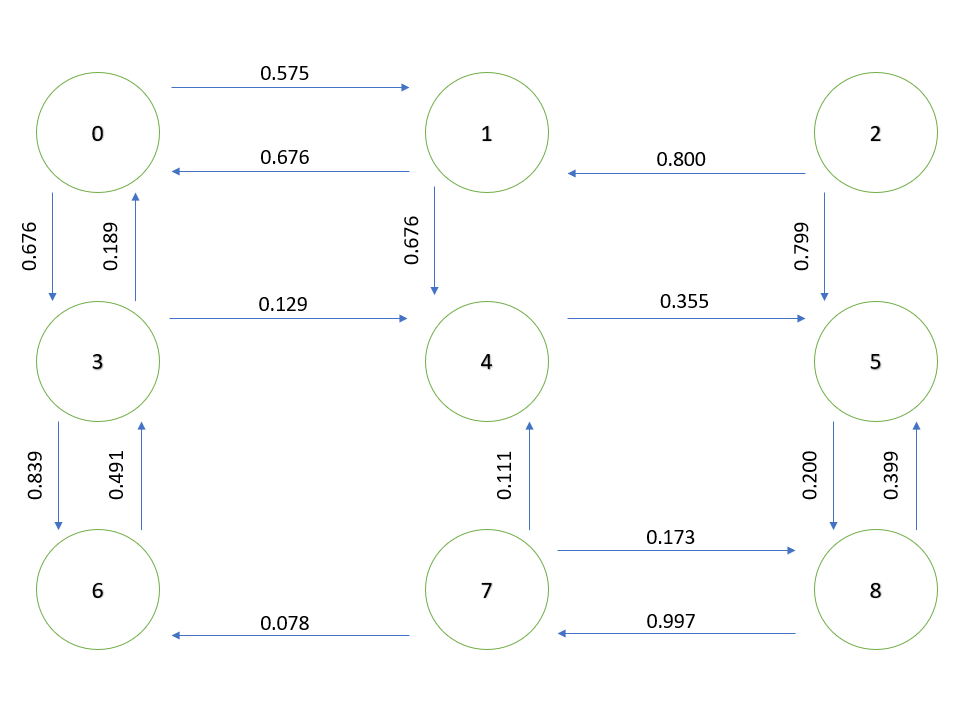
\includegraphics[width=1.1\textwidth]{graf2.PNG}
\caption{\textit{rys. 1 -- Graf przykładowy} \label{overflow}}
\end{center}


\section{Struktura katalogów}

\begin{itemize}
    \item Katalog główny w którym mieszczą się wszystkie pliki związane z projektem. Nazwa - \textit{Best Path}.
    \item Katalog \textit{img}, w którym będą się znajdowały wszystkie pliki graficzne. Katalog będzie się znajdował w folderze \textit{resources/com.example.best\_path}.
    \item Katalog \textit{fxml}, w którym będą się znajdowały wszystkie pliki o rozszerzeniu \textit{fxml}. Katalog będzie się znajdował w folderze \textit{resources/com.example.best\_path}.
    \item Katalog \textit{Controllers}, w którym będą się znajdować wszystkie kontrolery związane z obsługą interfejsu graficznego. Katalog będzie się znajdował w folderze \textit{java/com.example.best\_path}.
    \item Katalog \textit{Modules}, w którym będą się znajdować wszystkie klasy niezwiązane bezpośrednio z działaniem interfejsu graficznego. Katalog będzie się znajdował w folderze \textit{java/com.example.best\_path}.
\end{itemize}



\section{Wygląd interfejsu i jego funkcjonalności}

\begin{center}
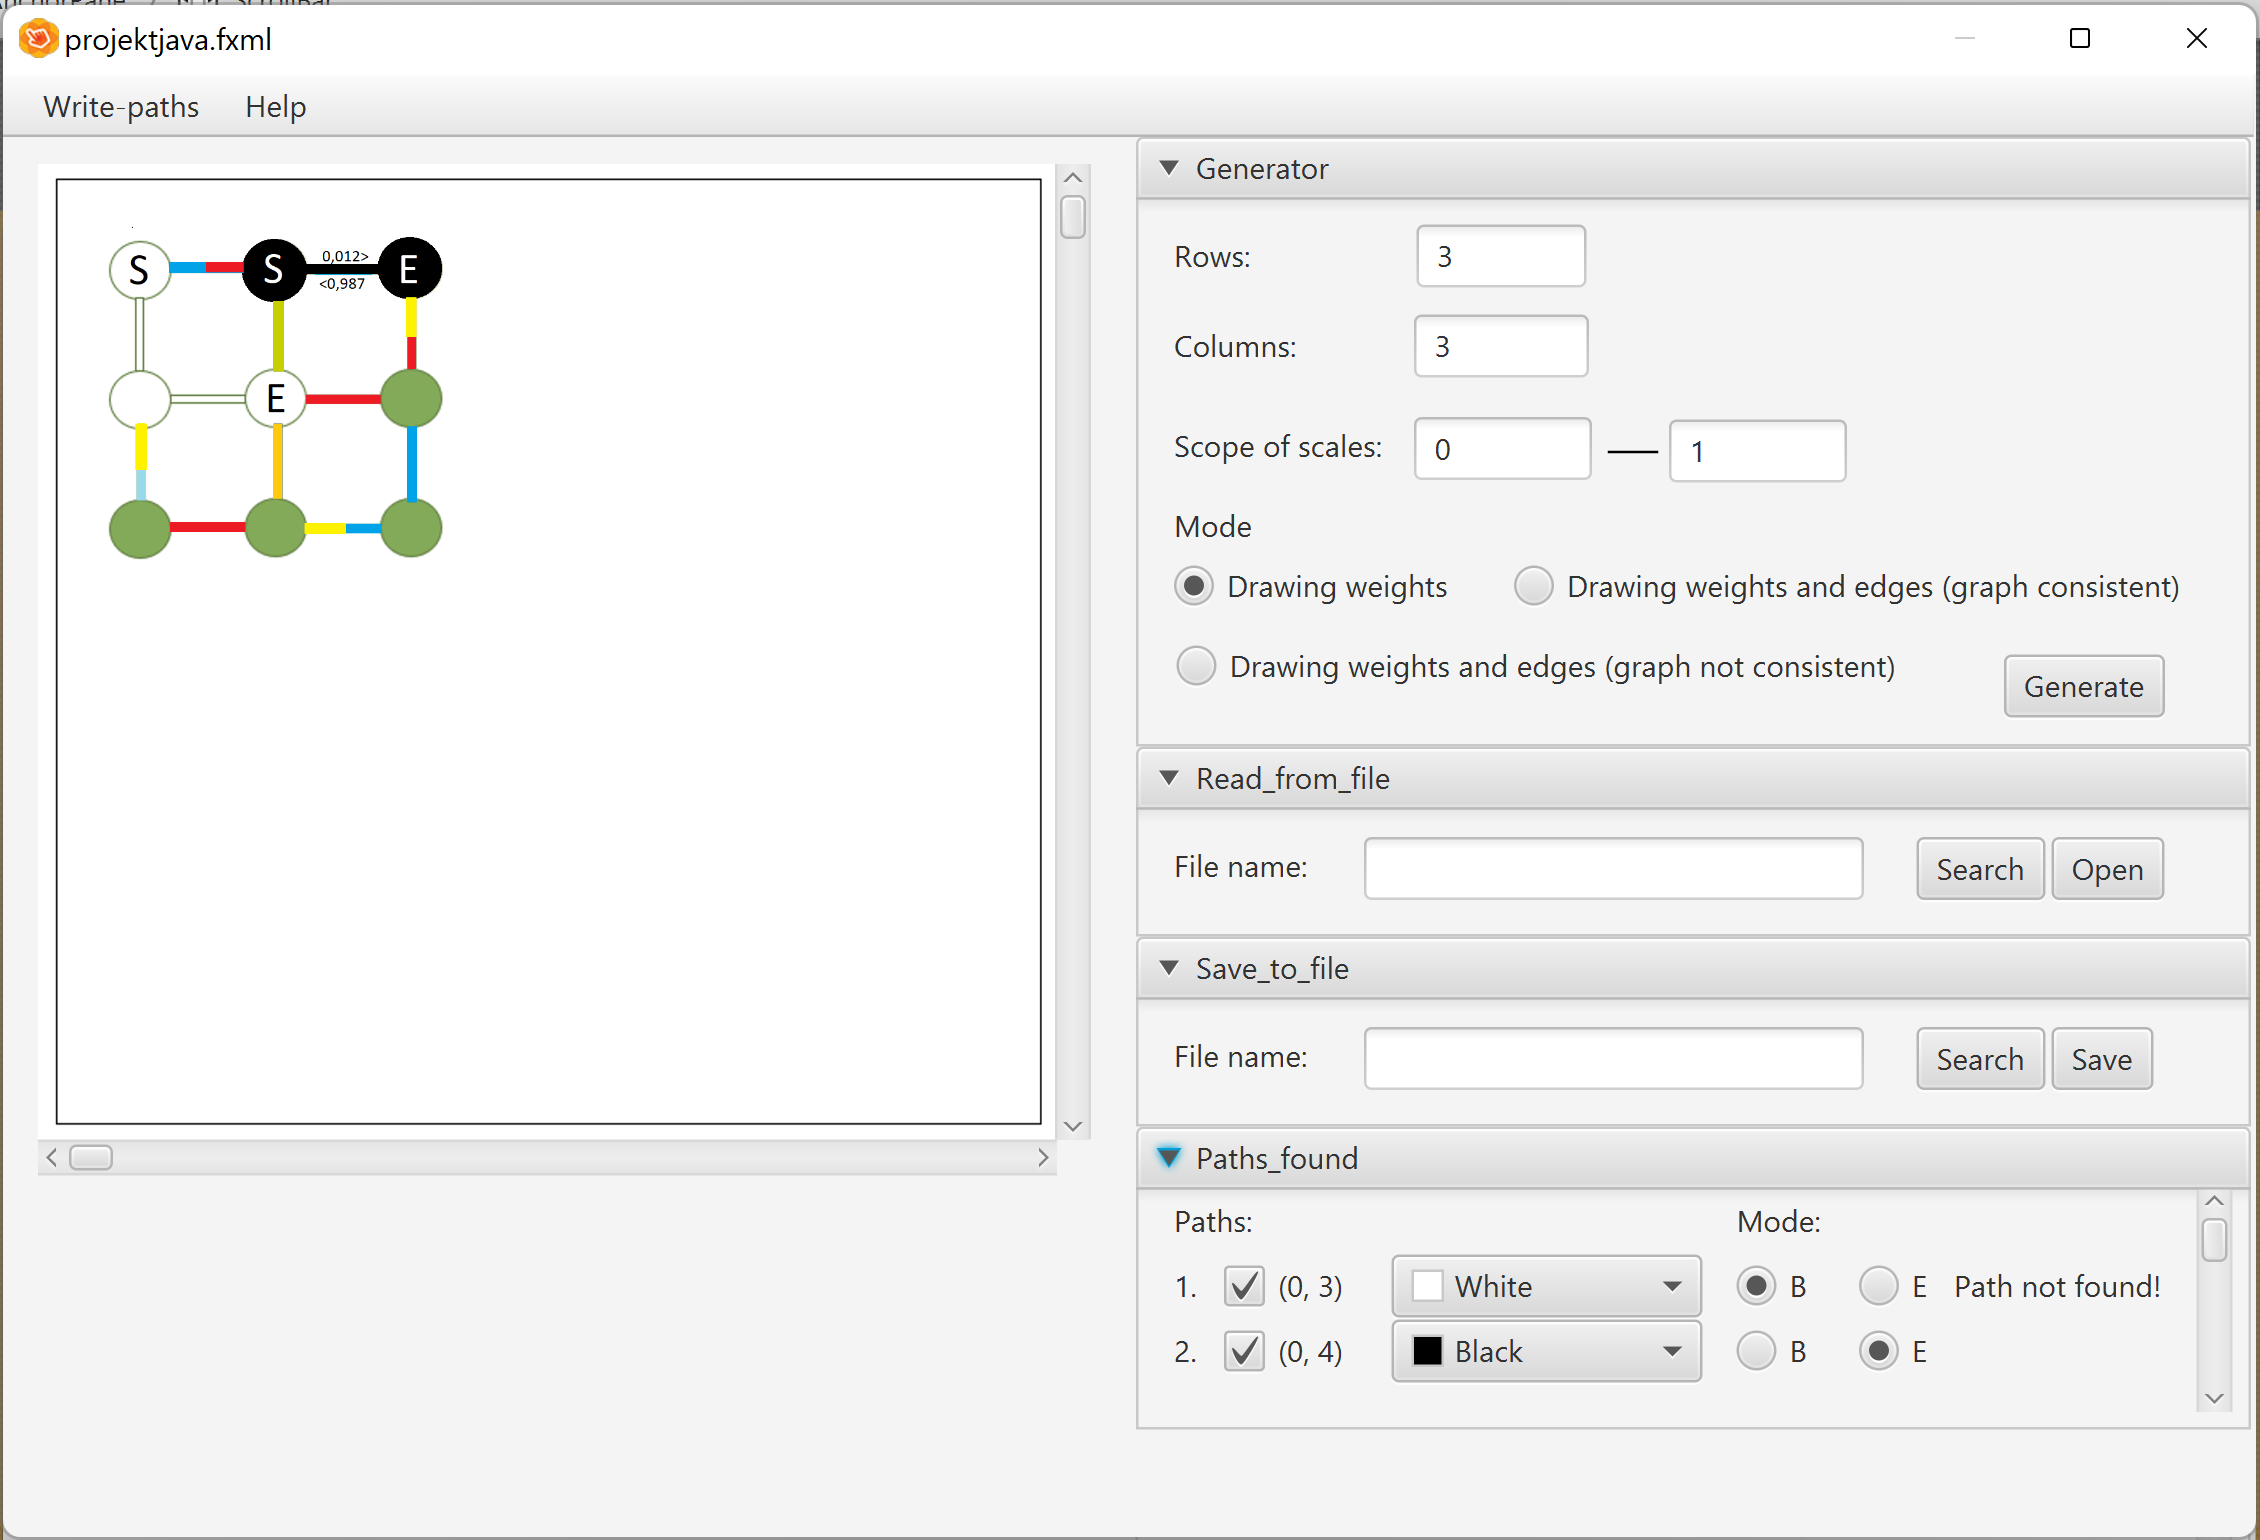
\includegraphics[width=1.1\textwidth]{JIMP JAVA/Prototyp GUI JIMP.png}
\caption{\textit{rys. 2 -- GUI (komunikat \texttt{Path not found!} został pokazany żeby było wiadomo gdzie się wyświetla i nie ma swojego odzwierciedlenia na wyświetlonym grafie (ścieżka $0->3$ istnieje)).} \label{overflow}}
\end{center}

Funkcje jakie będzie zawierał interfejs graficzny programu \textit{Best path}:
\begin{itemize}
    \item wyświetli graf (taki jak na rysunku \texttt{2 - GUI}), umożliwia powiększenie lub zmniejszenie grafu aby był bardziej czytelny. Jeżeli graf nie będzie się mieścił w oknie przeznaczonym dla grafu, pojawią się suwaki, które umożliwią przemieszczanie się po grafie,
    \item umożliwi wczytanie danych grafu z pliku o odpowiednim formacie,
    \item umożliwi wygenerowanie grafu w jednym z trzech trybów (podanych w podpunkcie\textit{Cel Projektu}), umożliwi również podanie zakresu wag oraz rozmiar grafu (tabelka \textit{Generator}),
    \item będzie również wyświetlał krawędzie pomiędzy wierzchołkami w kolorach od ciemno--niebieskiego do ciemno--czerwonego, w zależności od tego czy waga krawędzi jest bliska dolnej granicy wag czy górnej. Jeżeli droga z pierwszego wierzchołka do drugiego będzie inna od drogi z dugiego do pierwszego -- to wtedy krawędź będzie miała dwa kolory. Kolor odpowiadający wadze danego wierzchołka będzie znajdował się bliżej wierzchołka (patrz Rys. 2 \textit{GUI}),
    \item umożliwi wybranie wielu par wierzchołków za pomocą naciśnięcia myszką. Wierzchołek startowy będzie miał literkę \textit{S} na sobie, a~wierzchołek końcowy literkę \textit{E}. W celu odróżnienia par będzie można wybrać kolor wyświetlania danych par (tabelka \textit{Paths\_info}),
    \item umożliwi wyświetlanie znalezionej ścieżki, oraz umożliwi zmiane koloru wyświetlonych ścieżek w celu ich odróżnienia (wybór koloru pary to również wybór koloru ścieżki) lub całkowite ich zniknięcie. Jeżeli ścieżka nie zostanie znaleziona, zostanie wyświetlony odpowiedni komunikat przy wierzchołkach tej ścieżki (patrz Rys. 2 \textit{GUI}),
    \item jeżeli program natrafi na błąd związany z danymi podanymi przez użytkowika, wyświetli odpowiedni komunikat i pozwoli użytkownikowi ponowne wprowadzenie danych,
    \item umożliwi wczytanie danych z pliku wybranego przez użytkownika (\textit{Read\_from\_file}), plik będzie można wybrać za pomocą przycisku \textit{Search}, który otworzy eksplorator plików.
    \item umożliwi zapisanie grafu do wybranego pliku, plik będzie można wybrać za pomocą przycisku \textit{Search}, który otworzy eksplorator plików. (tabelka \textit{Save\_to\_file}),
    \item umożliwi wyświetlenie informacji za pomocą \textit{help}, który znajduje się w pasku menu programu. Umożliwi również wyświetlenie przykładowego pliku o poprawnym formacie.
    
    \begin{center}
    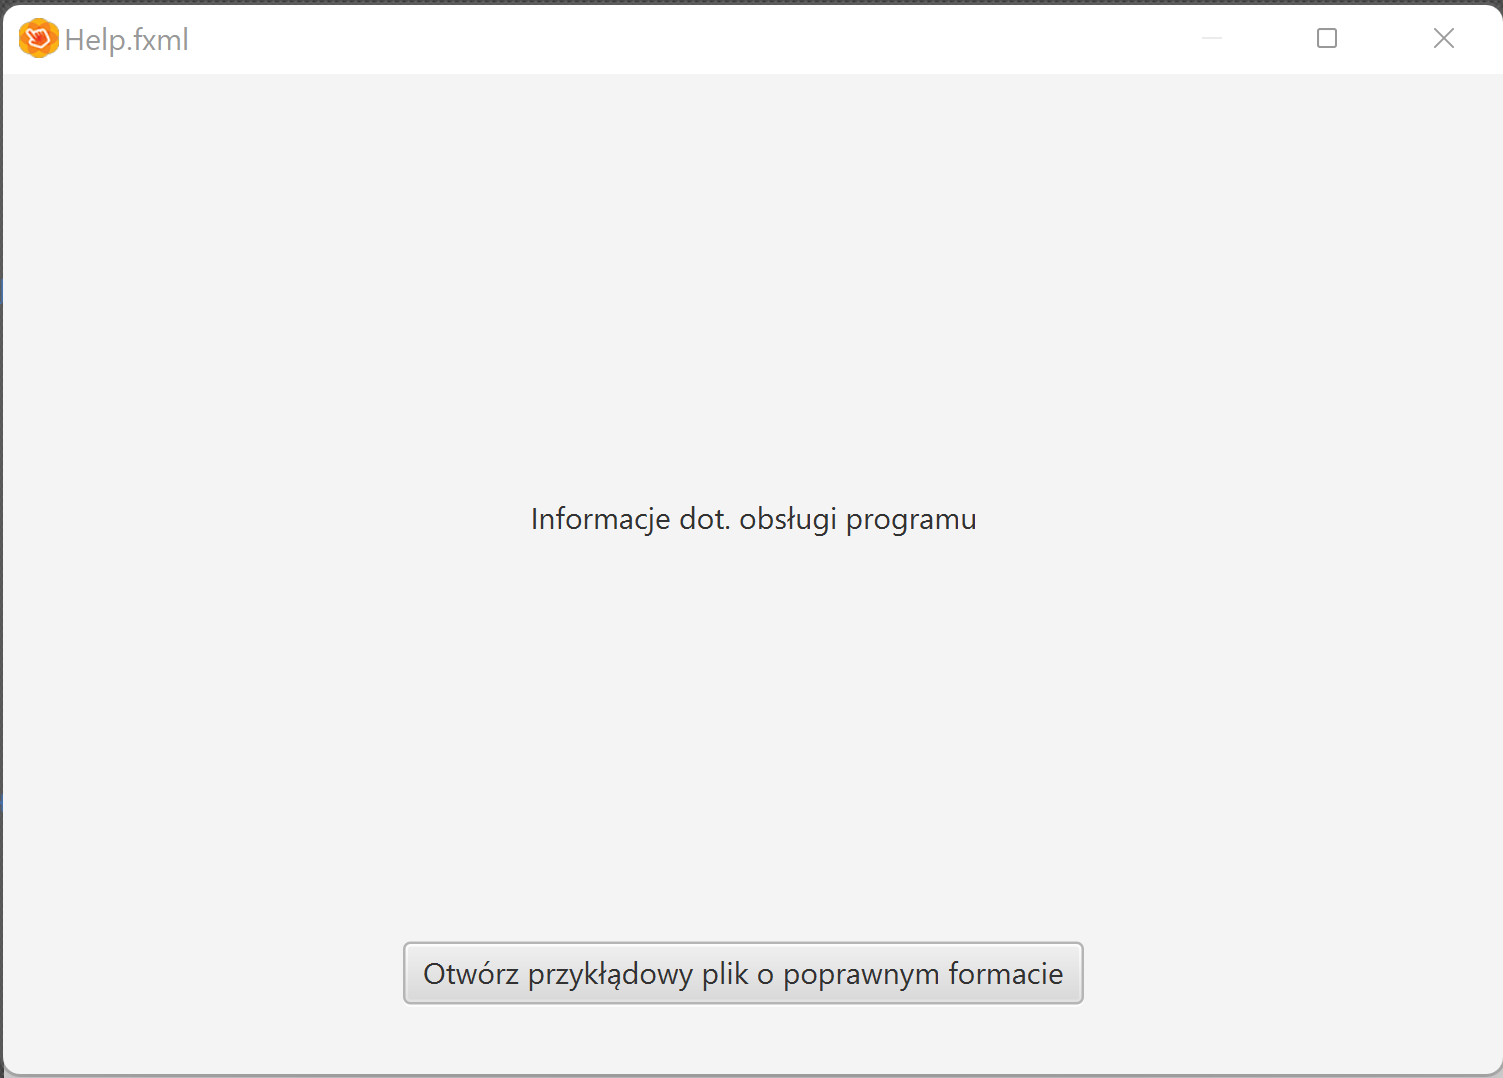
\includegraphics[width=0.5\textwidth]{JIMP JAVA/help_example.png}\\
    \caption{\textit{rys. 3 -- Przykładowy help} \label{overflow}}
    \end{center}
    
    
\end{itemize}


\section*{Komunikaty o błędach}

Program będzie w stanie wykryć wszystkie błędy spowodowane przez użytkownika oraz będzie komunikował wykrycie błędów poprzez komunikaty wyświetlane na ekranie.

\begin{center}
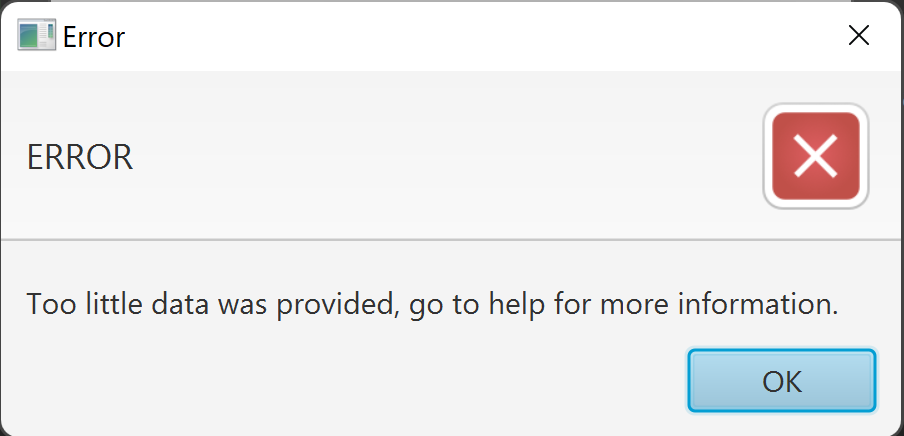
\includegraphics[width=0.5\textwidth]{JIMP JAVA/ErrorExample.png}\\
\caption{\textit{rys. 4 -- Przykładowy ERROR} \label{overflow}}
\end{center}

\\Komunikaty o błędach oraz ich wyjaśnienia:

\begin{itemize}
\item \texttt{Error: Incorrect data \-- [nazwa zmiennej], go to \textit{help} for more information.}\\\\
Błąd ten inforumje użytkownika o błędnym typie danych podanym do danej rubryki w interfejsie oraz podaje nazwy rubryk, w których błąd ten wystąpił.\\\\
(Np.: \texttt{Error: Incorrect data \–- scope\_of\_scales, go to \textit{help} for more information.}\\


\item \texttt{Error: Too little data was provided, go to \textit{help} for more information.}\\\\
Błąd ten inforumuje, że podana została zbyt mała ilość danych.
\item \texttt{Error: Problem occurred while opening given file, go to \textit{help} for more information.}\\\\
Błąd ten informuje, że wystąpił problem podczas otwierania pliku.
\item \texttt{Error: Given file has a wrong format, go to \textit{help} for more information.}\\\\
Błąd ten informuje, że podany plik ma nieodpowiedni format danych.

\end{itemize}



\section{Przykładowe użycie}
Do uruchomienia programu przygotowany zostanie plik \texttt{Best\_path.jar} za pomocą którego będziemy mogli wyświetlić okno naszego programu.\\\\
Program będzie umożliwiał wyświetlenie grafu na dwa sposoby tj. przez wygenerowanie nowego grafu za pomocą funkcji \textit{Generator} lub wczytanie grafu za pomocą funkcji \textit{Read\_from\_file}.
\subsection{Generowanie grafu za pomocą funkcji \textit{Generator}}
W celu wygenerowanie grafu za pomocą funkcji \textit{Generator} musimy podać liczbę wierszy i kolumn w rubrykach \textit{Rows} oraz \textit{Columns}, następnie w rubrykach \textit{Scope of Scales} podajemy zakres wag połączeń między wierzchołkami, a na końcu w sekcji \textit{Mode} wybieramy jeden z trzech trybów, w jakim nasz graf ma zostać wygenerowany. W przypadku podania danych o poprawnym formacie tzn. zgodnie z opisem podanym w sekcji pierwszej (\textit{Cel Projektu}), po naciśnięciu przycisku \texttt{Generate} na panelu po lewej stronie okna powinien wygenerować się graf zgodny z podanymi parametrami, jeżeli podane dane nie były zgodne z narzuconym formatem, to w takim przypadku pojawi się okno informujące o błędzie.
\subsection{Generowanie grafu za pomocą funkcji \textit{Read\_from\_file}}
Funkcja \textit{Read\_from\_file} jak sama nazwa wskazuje umożliwia wczytanie grafu z pliku podanego przez użytkownika. Ścieżkę do pliku możemy podać przez wpisanie jej do rubryki \textit{File name} lub przez wybranie go spośród folderów znajdujących się na naszym komputerze, po naciśnięciu przycisku \texttt{Search}. Mając wybrany plik z danymi otwieramy go za pomocą przycisku \texttt{Open}, jeżeli format pliku jest poprawny tzn. zgodny z opsiem podanym w sekcji (\textit{Problem}), to graf pojawi się na panelu po lewej stronie okna programu, w~innym przypadku pojawi się odpowiedni komunikat o błędzie.

\subsection{Znajdowanie i wyświetlanie najkrótszych ścieżek}
W celu wygenerowania najkrótszej ścieżki, należy wybrać wierzchołek początkowy oraz końcowy przez wciśnięcie ich myszką na panelu z wygenerowanym grafem, a następnie wcisnąć przycisk \texttt{Write\_paths} w lewym górnym rogu okna programu. Znaleziona ścieżka zostanie dodana do panelu \textit{Paths\_found}, jeżeli istnieje połączenie między wybranymi wierzchołkami, w przeciwnym wypadku szukane połączenie również pojawi się w tym panelu, ale z informacją, że nie znaleziono połącznia między wybranymi wierzchołkami.\\\\
Znalezione ścieżki zostaną zaznaczone na wygenerowanym grafie, jeśli zaznaczymy "tickbox" znajdujący się przy ścieżce, którą chcemy wyświetlić. Każdej znalezionej ścieżce przypisywany jest unikatowy, losowy kolor, który później może zostać zmieniony. Ostatnią funkcją dotyczącą wyświetlania jest wybranie trybu wyświetlania w sekcji \textit{Mode}. Do wyboru mamy tryb \textit{B}~(\textit{Basic}), czyli wyświetlanie samej ścieżki bez wag połączenia oraz tryb \textit{E}~(\textit{Extended}), czyli tryb rozszerzony, w którym oprócz ścieżki wyświetlane są również wagi.

\subsection{Zapis grafu oraz opcja \textit{help}}
W celu zapisania grafu, należy podać ścieżkę do folderu, w którym chcemy zapisać nasz plik panelu \textit{Save\_to\_file} w rubryce \textit{File name} lub wybrać go spośród folderów znajdujących się na naszym komputerze, po naciśnięciu przycisku \texttt{Search}. W przypadku próby zapisu bez wygenerowanego grafu, podania nieistniejącej ścieżki do folderu lub problemu z zapisem pliku, zostanie wyświetlony odpowiedni komunikat o błędzie.\\\\
W przypadku wystąpienia problemów z obsługą programu, lub chęcią zapoznania się z jego funkcjami, należy skorzystać z opcji \textit{help} znajdującej się w lewym górnym roku okna programu. Po wybraniu tej opcji wyświetlone zostanie okno z opisem działania programu.\\


Przykładowe użycie przedstawione jest w podpunkcie 4 ,,Wygląd interfejsu i~jego funkcjonalności" na rysunku 2 - ,,GUI".




\section{Testy akceptacyjne}
W celu sprawdzenia poprawnego działania programu, przygotowane zostaną testy akceptacyjne, które będą miały na celu:
\begin{itemize}
    \item Przetestowanie odporność na niepoprawność danych podanych przez użytkownika (plik do wczytania, plik do zapisania, dane do generacji grafu).
    \item Przetestowanie działania programu dla grafów o większych rozmiarach (czas działania).
    \item Przetestowanie poprawności działania programu (czy dane z pliku zostały poprawnie wczytane, poprawnie zapisane, czy została znaleziona poprawna ścieżka).
\end{itemize}






\end{document}